\documentclass[../main-v1.tex]{subfiles}
\begin{document}
\chapter{Databases \hideme{Buchanan and Laycock - draft}}
\label{ch:db}

%%%%%%%%%%%%%%%%%%%%%%%%%%%%%%%%
\section{Introduction  \hideme{Buchanan and Laycock - draft} }
\label{sec:db:intro} 

In order to accommodate the large range of metadata that will be tracked by \dword{dune}, the \dword{dune} \dword{db} structure comprises several databases specific to the information, or metadata, that they contain. 
The subset of all \dword{dune} metadata that is required, in the strict sense of being absolutely necessary, for data processing and analysis needs to be carefully identified and assessed.  We refer to this subset of metadata as "conditions metadata", see section \ref{subsec:db:conditions_metadata}.
It is critical that users be able to access conditions metadata throughout the full data processing and analysis chain with as little burden as possible. To achieve this, users will interact with a centralized high-level interface   described in Section~\ref{sec:db:conditions}.

The \dword{dune} experiment is expected to operate for 20-30 years and the \dword{dune} databases need to be reliably maintained and operated for that entire period. In order to accommodate this requirement, the database system should not rely on implementation solutions that possess the risk of becoming unavailable during the operation period. Open-source, non-proprietary solutions will therefore be used. Currently the databases housed at \dword{fnal} use the open-source PostgreSQL (Postgres) relational database management system. Postgres is supported by the \dword{scd}.       
\dword{dune} would also like to benefit from the close collaboration between \dword{doe} laboratories to improve service availability and mitigate single-point-of-failure risk by having secondary databases at other \dword{doe} labs.  \dword{bnl} is a good example of a lab that already provides database services to international experiments using the same Postgres technology.

It is expected that there will be reconstruction and analysis jobs distributed across large numbers of traditional grid-based and high-performance computing (\dword{hpc}) systems and that database access will need to be able to scale appropriately. Additionally, it is important to ensure that users are able to work on analysis tasks when unable to access the database directly through a network connection. 

Some of the database solutions outlined in this document have been deployed and tested to some degree during Run I of the \dword{protodune} experiment. Experience coming from %anne\dword{protodune} Run I 
this will be briefly described in the sections below, when relevant. %anneRun II of the 
The \dword{protodune2} experiment will provide a further testbed for the database systems proposed for DUNE.  

\subsection{Conditions Metadata}
\label{subsec:db:conditions_metadata} 

Conditions Metadata is defined as the information necessary to understand the context of physics data, e.g., beam data or calibrations.
%special run data
Metadata can be indexed by %anne either 
time, run, or fraction of a run (subrun). 
%Additionally, 
An \dword{iov}
%\dwords{iov2} 
defines the period, indexed by any of the three options, for which a given metadata is valid.
%may be used to index metadata that is used over periods not directly corresponding to run or subrun boundaries. 
Alignment constants are an example of conditions metadata that will likely be valid for several runs. 
The DUNE conditions database will have APIs that provide easy and transparent access to all conditions metadata independently of technical details.
%be indexed in a fashion that makes access by users transparent, or APIs will provided to serve the same purpose.

Time-indexed metadata will, in some cases, be sampled at a rate higher than typically needed by offline users. In these instances the metadata will be filtered down, or interpolated, to a lower rate for inclusion in the conditions database. In general, metadata falls into two categories, interpolated and non-interpolated, where an example of the latter would be run-indexed values pertaining to run configuration. Interpolated metadata, e.g., values read back from the slow control system, can be interpolated through a rolling average or updated on changes to the values. The method used will depend on the natural variation of the value being recorded and the physics use case. 
%I removed the user defining this, to stress that it should be a physics motivation
The database group will provide interpolated values to match the physics requirements of the experiment.  

Conditions metadata will in general be stored in appropriate databases but there will be some cases where it is more reasonable to include the metadata with the raw trigger records instead. An obvious example of this is metadata that changes at the individual trigger record level, i.e., trigger bit information. 

\hideme{Is this conditions metadata?  An example would be good.
%Some metadata that is appropriate for inclusion in a database may be naturally included in the raw trigger record data due to its being generated internally within the \dword{daq} during run initialization or during a run. This metadata will be extracted from the data during the reconstruction for inclusion in the appropriate database. 
}

The following table contains classes of metadata: 

\begin{comment} REDID BELOW - WAS TOO WIDE (ANNE) %%%%%%%%%%%
\begin{dunetable}
[Run Configuration Database Content]
{l l l l} 
%\begin{table}[ht!]
%\centering
 %\begin{tabular}{l l l l} 
 {table:metadata}
 {Example metadata values and types stored in the run configuration database.}
 Metadata  & Example(s) & Database &  Interpolated? \\ [0.5ex] 
 %
Run Configuration   &  Start Time, config file & Run Configuration & No\\  
Detector Conditions  & TPC high voltages & Slow Control & Yes  \\ 
Beam Conditions  &  Horn polarities, beam current & IFBeam & Yes \\  
Hardware Information & Component history &  Hardware/QC  & No \\  
Calibration Constants & Channel gains  & Calibration & No \\ 
Physics/Hardware Locations & Channel maps & Geometry & No \\  
Data Quality & Good runs list & \Dword{dqm} & No \\  
%
%\end{tabular}
%{Example metadata values and types stored in the run configuration database.}
%\label{table:metadata}
\end{dunetable}
\end{comment}
%%%%%%%%%%%%%%%%%%%%%%%%%%%%%%%%%%%

\begin{dunetable}
[Run Configuration Database Content]
{l l l} 
 {table:metadata}
 {Example metadata values and types stored in the run configuration database. (I) indicates interpolated metadata.}
 Metadata  & Example(s) & Database  \\ 

Run Configuration   &  Start Time, config file & Run Configuration \\   \toprowrule
Detector Conditions (I)  & TPC high voltages & Slow Control   \\ \colhline
Beam Conditions (I)  &  Horn polarities, beam current & IFBeam  \\ \colhline  
Hardware Information & Component history &  Hardware/QC   \\ \colhline  
Calibration Constants & Channel gains  & Calibration  \\ \colhline 
Physics/Hardware Locations & Channel maps & Geometry  \\ \colhline  
Data Quality & Good runs list & \Dword{dqm}  \\  
\end{dunetable}

A DUNE metadata task force was assembled in 2020 and a resulting report discussing the interfaces between online and offline systems can be found in reference~\cite{bib:docdb22983}.

\section{Conditions Database  \hideme{Buchanan and Laycock - draft}}
\label{sec:db:conditions} 

The conditions database is a high-level database that provides an interface to offline users and processes. The motivation for such a centralized database is to provide an easy-to-use interface for users and to reduce the number of database connections required by offline processes. This will ensure that jobs will be ``lightweight'' and processing time will not be extended due to database accesses. 
As the granularity and content of the conditions database should be well-matched to offline needs by design, it allows heavy use of caching technologies to optimize resource usage.  
The design of the interface between the data processing software framework (see chapter \ref{ch:fworks}) and the conditions database plays an important role if all of the access patterns needed by \dword{dune} are to be well supported.
Experience from other \dword{hep} experiments with distributed computing resources show that careful design of this interface is crucial to the success of the computing model
\footnote{Overlays (see section \ref{sec:usecases_overlays} are an example of a workflow that can cause issues for conditions database access if this interface is not well designed.}.
Figure~\ref{fig:dbmap} shows the relationship between the conditions \dword{db} and the other \dword{dune} databases. For \dword{protodune} the "Master Metadata Store" is an intermediate database that allows for potentially heavy data interpolation tasks to run without creating extra load on the other, often critical, database services.  It provides separation between the online and offline worlds at the cost of partial data duplication. The final database system design for \dword{dune} will benefit from experience with this design.


\begin{dunefigure}
[Map of DUNE databases]
{fig:dbmap} 
{Map of DUNE databases showing conditions database (combination of Master Store and Run Conditions DB). The arrows illustrate the flow of metadata. Offline access to conditions metadata is made through the Run Conditions DB, which is a relational DB containing a small subset of the metadata from the Master Store DB. }
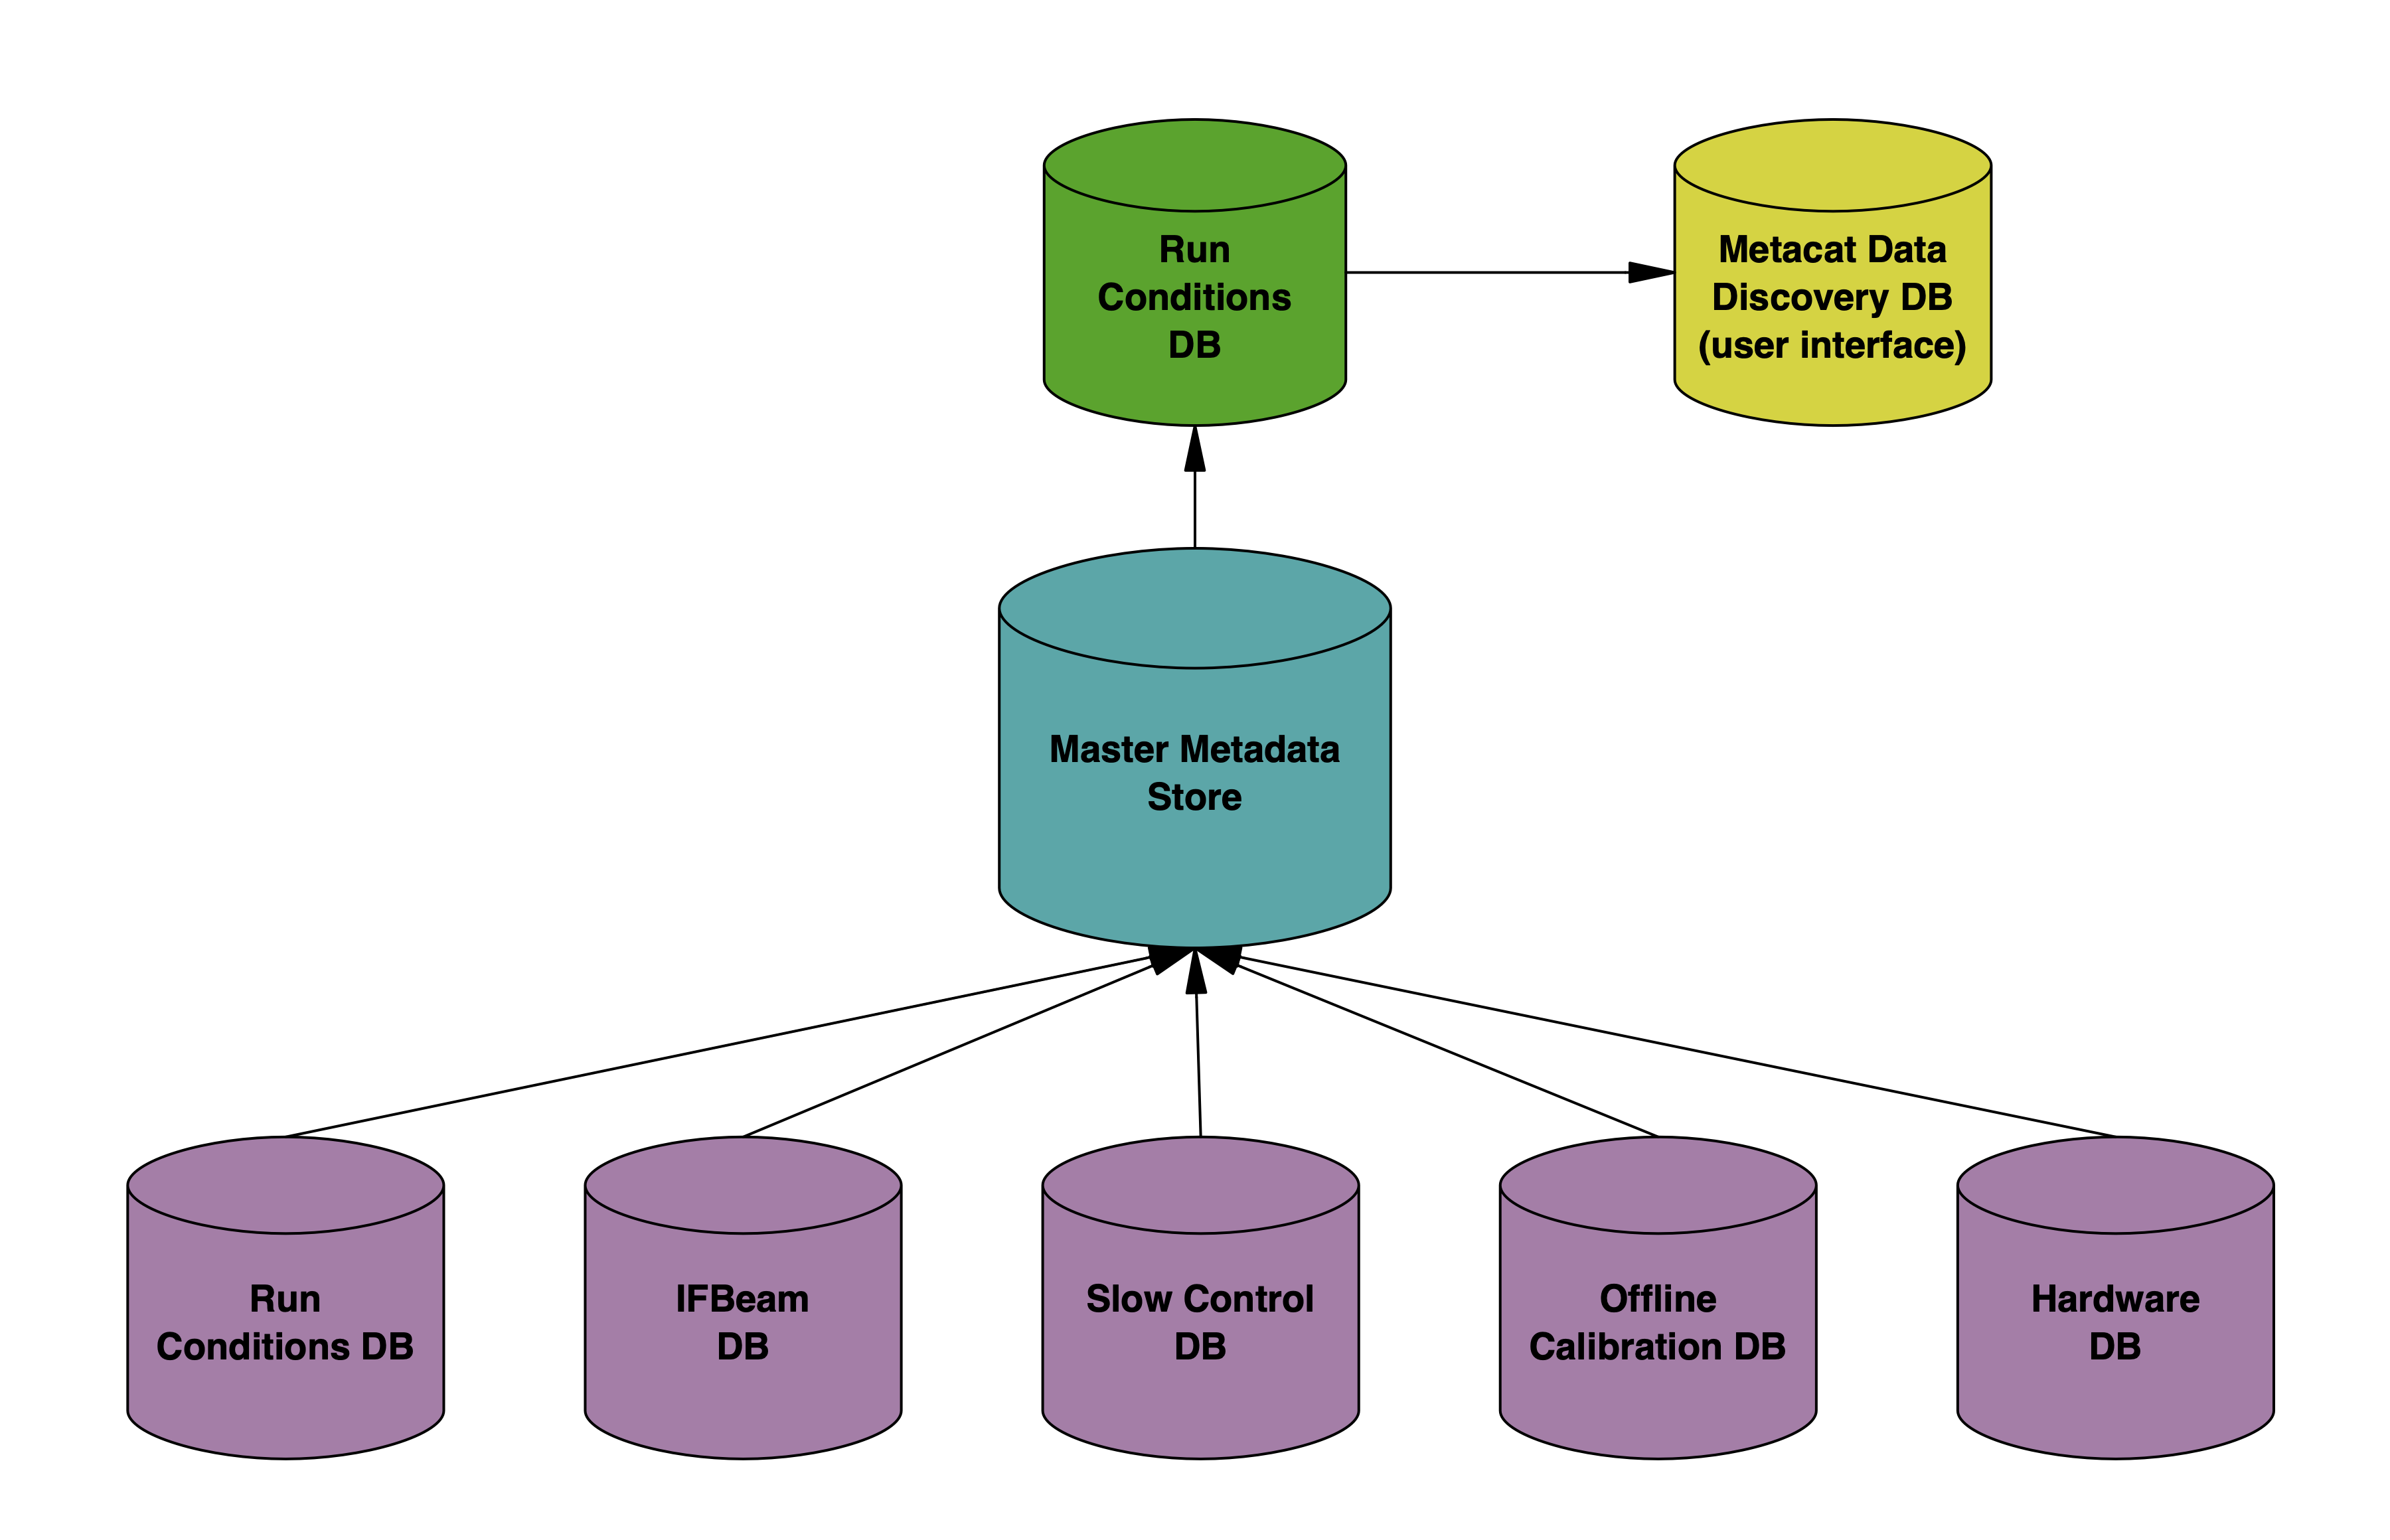
\includegraphics[width=.9\columnwidth]{graphics/Databases/DBSystem-cartoon.png}
\end{dunefigure}

The conditions database will contain interpolated (e.g., slow controls) and non-interpolated (e.g., run configurations) information. Interpolated information may more naturally be keyed by time-stamps, while configurations are more naturally keyed by run number. Tools will need to be developed to handle these two  
types of database content. 

\subsection{Conditions Database for \dword{protodune}}

In order to provide a balance between the availability of the largest set of metadata possible  and allowing schema evolution,  the \dword{protodune} conditions database will employ an unstructured approach utilizing a No-SQL database \dword{ucondb}~\cite{bib:ucondb}. The \dword{ucondb} where metadata from several specific databases and sources, like the \dword{daq} system, will be stored in ``blobs'' corresponding to temporal periods (run, time blocks, or \dwords{iov2}). Each blob will contain a \dword{json}-formatted record of metadata. Folders will be used to hold metadata corresponding to time and run keys. Tools will be provided to correlate between the two. 

An example of a metadata blob~\footnote{This metadata is taken from \dword{iceberg}, a small DUNE-related experiment. \dword{protodune}, and DUNE, conditions metadata will be significantly larger, O(10~MB).}

\todo{THIS NEEDS TO BE UPDATED}
\begin{verbatim}
{
    "Run Number": 648,
    "Start Time": " 2019-03-04T22:23:40",
    "End Time": " 2019-03-04T22:25:31",
    "Pulser Mode": 2,
    "Pulser DAC": 7,
    "Gain": 2,
    "Shaping": 2,
    "AC Coupling": 0,
    "Baseline High": 1,
    "Leak High": 1,
    "Leak 10x": 0,
    "FE Buffer": 0,
    "Events": 228,
    "Filename": " iceberg_r000648_sr01_20190304T222340_1_dl1.root",
    "isduplicate": 0,
    "DAQ Config": "iceberg_g2s2b1_maskWIB001FEMB4_pulser7_00001"
}
\end{verbatim}

%A smaller relational database will contain a subset of the metadata most often queried by users. This will enable much faster queries than accessing the unstructured conditions database directly.

\subsection{Conditions Database for DUNE}

For \dword{dune}, the interface between the conditions database and the software framework will become particularly important.  The consensus among several \dword{hep} experiments was reported in an \dword{hsf} whitepaper \cite{Laycock:2019ynk}. Here, a lightweight relational database schema allows a single point of entry, a "global tag", to configure conditions data access for the framework.  Evolving the \dword{protodune} solution to benefit from that experience is foreseen by the database group. Further details on the development plan can be found in section \ref{sec:db:conddbdev}.

%An unstructured conditional database was used for the \dword{protodune} experiment. Collections of metadata corresponding to \dword{protodune} runs were stored as text-based ``blobs'' in key-value pairs. For the first \dword{protodune} run the blobs contained \dword{fhicl}-formatted information and Run II blobs will be in \dword{json} format. The \dword{ucondb} format enables the capture of a comprehensive set of metadata without the need for a strict schema to be determined in advance of operating the database. Postgres provides the ability to utilize folders in the database structure, which can be used for versioning should the metadata coming from any source change over time. Folders can also keep metadata keyed by run number separate from that keyed by time. Tools can be used to match either up to any \dword{iov2}-based query. Further details of the use of the \dword{ucondb} for \dword{protodune} can be found in Section~\ref{sec:runconfigPD} 

\section{Run Configuration Database  \hideme{Buchanan and Laycock - draft}}
\label{sec:db:config}  

The run configuration database contains the intended configuration of the detectors and \dword{daq} during data collection -- physics or otherwise. 

Metadata contained in the run configuration database includes hardware settings, run type, and run start and end times. Table~\ref{table:runconfig} contains some examples of typical metadata that will be contained in the run configuration database. 

\begin{dunetable}[Run configuration database example]
{l  l } 
{table:runconfig}
{Example metadata values and types stored in the run configuration database.}
%\begin{table}[h!]
%\centering
% \begin{tabular}{l  l } 
% 
 Metadata Value & Type  \\ [0.5ex] 
 
Start of run   &  Time \\ \toprowrule
Readout window size  & Integer  \\ \colhline
Readout trigger type  &  Integer \\  \colhline
Readout firmware version &  Integer \\  \colhline
Baseline start &  Integer \\  \colhline
Shifter comments &  Text \\  \colhline
Run end status & Integer \\  
%
%\end{tabular}
%\caption{Example metadata values and types stored in the run configuration database.}
%\label{table:runconfig}
%\end{table}
\end{dunetable}

The majority of run configuration metadata comes from the configuration files used by the \dword{daq} system during run execution. Some additional metadata collected at the end of the run, or shortly thereafter, may also be included. Examples are run completion status and comments made by the shifter during the run or in run-related checklists.

Parameters used to configure the run will be collected and packed into \dword{json}-formatted blocks in a single blob corresponding to a \dword{daq} run.   

\subsection{Run Configuration Database for ProtoDUNE}
\label{sec:runconfigPD}

 Following the completion of a run, the run configuration parameters corresponding to the run are read from the mongoDB and packed into a single %anne"blob" 
 blob of key-value pairs in \dword{json} format. Any additional information, such as end-of-run time, are added to the blob, which is then transferred to the \dword{ucondb} at \dword{fnal}. A typical metadata blob is on order 10\,MB in and contains more information than most users will want to use. An additional step of reducing the metadata is performed to produce a subset of metadata needed by offline users. The reduced set of metadata is stored in a single table in a relational database referred to as the ``run history database.'' An interface is provided to users, enabling them to retrieve run numbers and file locations based on queries of the history database. 

For %anne Run II of 
\dword{protodune2} the conditions \dword{db} will include metadata from multiple sources, as will be the case for DUNE. Metadata from the beam conditions database (IFBeam), the slow controls database, and data quality monitoring database (DQMDB), will be included in addition to the run configuration information. The \dword{ucondb} is able to store data keyed by either non-interpolated values (run number) or interpolated values (timestamps). Users are then able to access information using run numbers or dates and times.

\begin{dunefigure}
[Flow of metadata from \dshort{protodune} DAQ to user interface]
{fig:protoconditions} 
{Flow of metadata from \dword{protodune} \dword{daq} to user interface.}
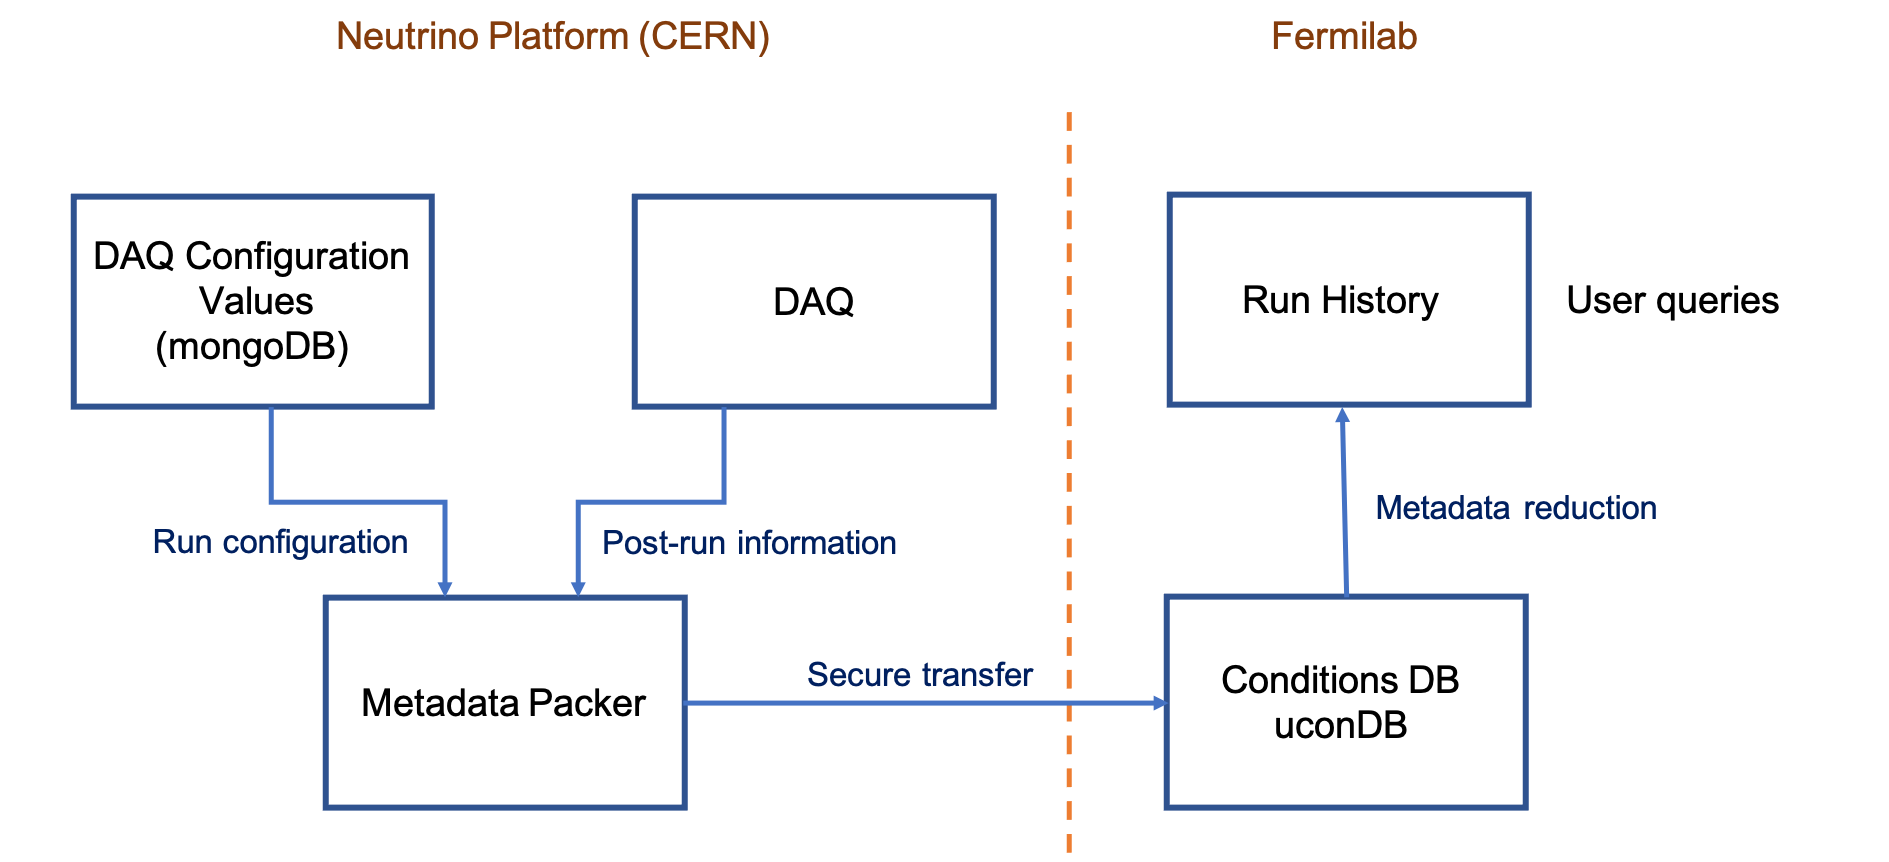
\includegraphics[width=.9\columnwidth]{graphics/Databases/Conditions_ProtoDUNE.png}
\end{dunefigure}

\section{Data Quality and Monitoring Database  \hideme{Buchanan and Laycock - draft}}
\label{sec:db:dqm}  

The \dword{dqmd} contains monitoring histograms and metadata derived from data collected during operation of the DUNE detectors. The \dword{dqmd}  is an online database and
the histograms it stores to assess and monitor data quality are critical for the operations of \dword{dune}, but not relevant for offline data processing and analysis.
The derived data quality metadata, which include boolean flags indicating the results of the online data quality assessment algorithms, are relevant for offline analysis and this small subset of \dword{dqmd} data will require an interface with the conditions database either directly or via an offline replica of the data quality database. \todo{ (anne) \dword{dqm} db?}

\section{Offline Calibration Database  \hideme{Buchanan and Laycock - draft}}
\label{sec:db:calib} 

The calibration database contains calibration constants determined from collected data corresponding to  \dwords{iov2}. The conditions metadata from the calibration system will result from offline calculations using data collected from the DUNE detectors.
There will generally be multiple versions of calibration constants corresponding to the same \dword{iov}, and the conditions database will provide coherent access to the appropriate version of these calibrations via e.g. the global tag mechanism.
%These versions will be contained within the database and accessible to users.  

\section{Slow Control Database \hideme{Buchanan/Laycock - draft}}
\label{sec:db:slowcontrol}  

The slow control \dword{db} contains metadata specific to the state of detectors during the time data were collected as well as before and after. Examples of slow control metadata are measurements of power supply voltages and currents, and temperatures. Each slow control quantity corresponds to a particular device. The slow control \dword{db} metadata is time-indexed and hence must be interpolated. Additionally, different devices will be sampled at different rates.

The slow control metadata is captured via a Supervisory Control and Data Acquisition (\dword{scada}) system that is the responsibility of the Slow Control and Monitoring group. The \dword{scada}  system pushes values to a back-end database, where the \dword{db} flavor is tied to the \dword{scada} solution. 
The \dword{scada}  system can provide data reduction through filtering prior to insertion of metadata into the back-end \dword{db}, which reduces the workload on any API used to move the metadata to the conditions database. 

\subsection{Slow Control Database for ProtoDUNE}
\label{sec:slowcontrolPD}

The \dword{protodune} experiment has been using an Oracle~\footnote{Oracle\textcopyright, \url{https://www.oracle.com}} back-end \dword{db} for the slow control system. As 
\dword{scd}
%Fermilab Scientific \todo{(anne) did you mean Core? }Computing Division 
does not support Oracle, the information from the Oracle database must be extracted and moved into a Postgres \dword{db} at Fermilab. Any filtering of the metadata not handled by the \dword{scada}  system when populating the Oracle database can be handled by the API that transfers the Oracle records to Postgres.

No data filtering was provided by the \dword{scada} system for \dword{protodune} Run I but for Run II it is expected that the slow controls conditions metadata will be filtered based on the physics needs.

\section{Beam Conditions Database - IFBeam  \hideme{Buchanan and Laycock - draft}}
\label{sec:db:ifbeam}  

The beam conditions database, \dword{ifbeam}~\cite{ifbeam} will contain metadata related to the condition extracted beam and corresponding diagnostics.  The functional form of this database is essentially the same as that of the slow control database. A large number of devices are sampled into the \dword{ifbeam} \dword{db}. The \dword{ifbeam} metadata transferred to the conditions \dword{db} will be a coarser subset of the original set.

Quantities contained in the \dword{ifbeam} \dword{db} include beam currents, horn currents and polarities, and beam monitoring instrument metadata.

\begin{dunetable}
[Example IFBeam metadata]
{l  l } 
{table:ifbeam}
{Example metadata values and types stored in the \dword{ifbeam} database.}
%\begin{table}[h!]
%\centering
% \begin{tabular}{l  l } 
% 
 Metadata Value & Type  \\ \toprowrule [0.5ex] 
% 
Horn 1 Polarity &  Integer \\ \colhline
Horn 2 Polarity  & Integer  \\ \colhline
Beam current & Float \\  
%
%\end{tabular}
%\caption{Example metadata values and types stored in the run configuration database.}
%\label{table:ifbeam}
%\end{table}
\end{dunetable}


\section{Hardware Database  \hideme{Buchanan and Laycock - draft}}
\label{sec:db:hwdb}  

The principle purpose of the hardware database (\dword{hwdb}) is to track the lineage of hardware components and record the results of their \dword{qc} tests. In this context a component can be a sub-detector module or any of the individual parts comprising it. For example, a readout board is a component as is a mezzanine daughter board or programmable logic chip mounted on the readout board. The lowest level component tracked within the \dword{hwdb} will be unique to the corresponding hardware system. 

A requirement of the \dword{hwdb} is that any component, or part, stored in the database must have a unique identification number assigned to it, coordinated by the \dword{dune} Integration group. % Jim Stewart 
%A separate database, under the responsibility of the DUNE Integration group, 
%\todo{(anne) is this a formal group, and is this the title?} will be the source of the unique part ID numbers assigned to each component. 
The part numbers will be designated as shown in Table~\ref{table:partsid}. The project field corresponds to DUNE detectors (D), integration (I), LBNF (L), and future project (P). The project identifier is allocated by the project management team while the other identifiers are left for the various hardware consortia to assign. There are additional fields not listed as they are not relevant to the \dword{hwdb}.  More details of the parts identification number can be founds in~\cite{bib:cernedms2505353}.

\begin{dunetable}
[Hardware database component IDs]
{l l l l l l} 
{table:partsid}
{Unique parts identification number assigned to each component stored in the hardware database.}
Project & System ID & Subsystem ID & Item Type ID & Dash & Item Number  \\ \toprowrule 
D/I/L/P & 01-99 & 001-999 & 00001-99999 & - & 00001-99999 \\  
\end{dunetable}

Hardware \dword{db} metadata will reflect the complete lifetime of the detector component, including the following:

\begin{itemize}
\item Procurement, 
\item Fabrication,
\item Quality control testing,
\item Shipping and storage,
\item Installation, and
\item Maintenance. 
\end{itemize}

The relationships between components will be reflected in the \dword{hwdb}. Metadata corresponding to multiple instances of events such as \dword{qc} tests will be handled using time series within the database. 

The database group will provide an interface to the \dword{hwdb} and each hardware consortium will be required to ensure that their metadata is inserted into the database. Given the wide range of hardware consortia, the international nature of the experiment and the fact that individual consortia must manage their own construction projects, it is 
beyond the scope of the database group to dictate how the consortia will handle data entry into the \dword{hwdb}.  Instead, the database group will consult with the consortia, and in particular their database group liaisons, providing documentation for the \dword{hwdb} and advising on efficient methods for working with it.  Sharing of tools will be very strongly encouraged to reduce the duplication of effort as far as possible.
%expected that the various consortia will develop different metadata capture and temporary storage solutions. The database group will consult with the consortia but ultimately the consortia will need to provide their own APIs for record insertion into the \dword{hwdb}.  


\section{Service and Maintenance  \hideme{Buchanan and Laycock - draft}}
\label{sec:db:service}  

Most, if not all, of the DUNE databases will operate in advance of the full DUNE experiment coming online and these databases will need to be maintained and serviced once they are operational. 

The second run of the \dword{protodune} experiment (\dword{protodune2}) will employ a suite of databases that will be the precursors to the full database system that will be in place for DUNE. Each of these databases (run configuration, beam instrumentation, conditions, slow controls, and hardware) will require stable monitoring, maintenance, and service to address operational issues that will arise in the lead up to and during %anne the running of the \dword{protodune} II experiment. 
\dword{protodune2} operations.

Monitoring will be achieved using automated web-based tools \todo{[ref needed]|} and responses to offline database issues will be made within an 8-hour period corresponding to a typical operation or production ``shift'', i.e. 5 days a week
\footnote{The assumption is that offline database services will not require 7 days a week coverage.}
. For \dword{protodune2} databases will be located at both \dword{fnal} and \dword{cern}, both of which have a long history of database support.  Moving on to \dword{dune}, the expectation is that another \dword{doe} lab like \dword{bnl} would share database operations with \dword{fnal}.

\section{Development Plans  \hideme{Buchanan and Laycock - draft}}

There are a number of database-related projects where R\&D is needed or underway, utilizing effort \todo{how to credit the FOA funding???}
and expertise from both \dword{doe} labs and universities.  Coordination is provided by the Database group and attempts to balance the short-term needs of \dword{protodune} with the longer term needs of \dword{dune}.

\subsection{Conditions Database Development}
\label{sec:db:conddbdev}

The Conditions Database is the primary interface to conditions metadata for all \dword{dune} distributed computing resources and this task includes designing and developing caching strategies.  The \dword{dune} Database group will collaborate with the \dword{hsf} to benefit from the experience of other \dword{hep} experiments, as well as the experience gained from \dword{protodune}, to develop a robust system while optimizing development effort.

\subsubsection{Conditions Database Core Design}

The \dword{hsf} Conditions Databases group identifies the following points as key features of a good Conditions Database design:

\begin{itemize}
    \item    Loose coupling between client and server using RESTful interfaces
    \item    The ability to cache queries as well as payloads
    \item    Separation of payload queries from metadata queries
\end{itemize}

These guiding design principles are likely to remain valid throughout the lifetime of \dword{dune}, while implementation will need to evolve with technology.

\subsubsection{Conditions Database and Software Framework}

The interface between the Conditions Database and the Software Framework is defined by the Application Programming Interface (API) % let's see if we reuse this and it motivates a dword!
of the Conditions Database.  The \dword{hsf} Conditions Database group is in the process of defining a generic API, again using the experience of existing \dword{hep} experiments to understand best practice for supporting all read and write use cases.  \dword{dune} will collaborate with the \dword{hsf} on this API definition and share experience on implementations.  It is noted that, in line with the \dword{hsf}, given the heterogeneity of compute hardware that \dword{dune} needs to use, a common implementation is considered to be less important than a common API and sharing experience.

\subsubsection{Conditions Database Service Robustness and Distributed Computing}

In addition to the cache-friendly design of the central Conditions Database service itself, a major issue for a critical (for offline) service like the Conditions Database is resilience such that a robust and reliable service can be provided.  Here, \dword{dune} plans to take advantage of synergies with other \dword{doe} labs, particularly at \dword{bnl} which hosts Conditions Database services for Belle II and other experiments.  The backend database technology (Postgres) is common between \dword{fnal} and \dword{bnl}, and generally Conditions Database services, under the umbrella of the \dword{hsf}, are expected to evolve to look more and more similar.  \dword{dune} will investigate the potential for having a first class backup service (that would support writing as well as reading functionality), in addition to having redundancy of read functionality via intelligent use of caches at sites.


\subsubsection{Database Access for High-Performance Computing Facilities}

As DUNE will utilize \dword{hpc}   facilities for some analysis tasks it is important that \dword{db} access is manageable when tens, or hundreds, of thousands of processes are distributed across an \dword{hpc}   cluster. Studies on how scaling on such systems can be handled without overwhelming the conditions \dword{db} with an enormous number of simultaneous queries are required. %anne need to be undertaken. 
Here again, \dword{dune} plans to leverage the experience of other \dword{hep} experiments with experience of using \dword{hpc}'s at scale.

\subsection{Payload Serialization}

Similarly to the discussion in chapter \ref{ch:format}, the data format of conditions metadata deserves careful attention to avoid problems including technology lock-in.  The need to interact with many different groups, essentially all providers of conditions (and other persistent) metadata, is the main driver of the amount of effort required for this task.

\subsection{Slow Control Database Development}

The \dword{scada}  system chosen for Run I and II of the \dword{protodune} experiment was WinCC with Oracle as the back-end \dword{db}. This system is well tested and it is relatively trivial to transfer information from the Oracle \dword{db} to a \dword{postgres} \dword{db} located at \dword{fnal}. Given the fact that Oracle-based \dwords{db} are not guaranteed to be supported for the life of DUNE it would be beneficial to use a solution that enables a \dword{postgres} back-end.  The \dword{scada} system for \dword{dune} may also bring new challenges and the Database group are investigating potential solutions in collaboration with Slow Controls experts. 


\subsection{Hardware Database Development}

The core functionality of the Hardware Database is described in section \ref{sec:db:hwdb} and the first version is expected to be complete in FY22.  Experience gained as the consortia use the database are expected to motivate feature requests, many of which will require urgent attention to support the construction phase of \dword{dune}.  Looking further ahead, some attention will be needed to ensure the maintenance of this crucial database for the long lifetime of the collaboration.  Some information in the Hardware Database will correspond to Conditions Metadata (calibrations), thus requiring the transfer of data while retaining provenance.


\subsection{Run Configuration Database Development}

Transfer of Run Configuration information for offline use was a major problem for \dword{protodune} Run I, and significant effort will be used to improve the situation for Run II.  The evolution of both the \dword{dune} Conditions Database and \dword{daq} system could imply a similar amount of effort moving to \dword{dune}.


\subsection{Other Database Development}

The \dword{dune} Calibration system is expected to generate very large datasets that will be processed to create Conditions Metadata that needs to be transferred to the Conditions Database.  Meanwhile the Beam Conditions Database stores far more data than needed for the data processing Conditions Metadata, and effort will be needed to find efficient solutions for data reduction.  Finally, the Data Quality Monitoring Database is under the control of the \dword{dqm} group, with some amount of data needing to be transferred to the Conditions Database.  All of these connections could imply additional development work which, if arising from offline-only constraints, would should be supported by Database group effort.


\subsection{Database Access Tool Development and Documentation}

Guided by use cases, tools will be developed for all of the \dword{dune} Databases to enable to access of metadata for inclusion in the conditions database as well as direct access for studies\footnote{Most offline DB access will be made via the Conditions DB but there will be cases where expert users will need direct access to the various databases.}. An interface within the ART framework is already part of the DUNE software stack and has been used to access the IFBeam beam instrumentation database. This ART database service has been used, and is currently used, by the NOvA experiment. This interface will be the baseline for any other interfaces used by users interacting with the DUNE databases, including with the Conditions DB.

Additionally, APIs will be developed to provide the interfaces between the various databases and the Master Store DB, as well as between the Master Store and the Run Condition database. These will likely be light-weight Python-based applications. 

%As more use cases and workflows are discovered, all of the \dword{dune} Databases will likely need to have tools to allow efficient and easy access to them. 

Documentation is another critical aspect of the database system. This includes descriptions of the DB system components and training materials, that will need to be updated as development work proceeds. The number of use cases, databases and groups involved drive the significant amount of effort required here.


\subsection{Person Power Estimates}

The personnel needs will be largely front-loaded as the database systems are researched, implemented, and tested. The databases requiring the most effort will be the slow control, run configuration, calibration, and conditions databases.  

Estimates of the personnel needs over the next three years are given in Table~\ref{table:dbneeds}. 

\todo{PJL 03/15 - check these effort levels vs tasks looks somewhat sane}
\begin{dunetable}
[Person-power estimates for database development]
{l l}
{table:dbneeds}
{Database group R\&D person-power needs (FTE years) from FY22 to FY27.}
% \begin{table}[h!]
% \centering
%  \begin{tabular}{l l l l l} 
 
 % Assume we will mainly need to justify out to 2027 when there is a ramp down
 Task & Effort (FTE years) \\ \toprowrule
 
Conditions \dword{db}             & 6 \\ \colhline
Payload Serialization             & 4 \\ \colhline
Slow control \dword{db}           & 2 \\ \colhline
Hardware \dword{db}               & 2 \\ \colhline
Run Configuration \dword{db}      & 1 \\ \colhline
Calibration \dword{db}            & 1 \\ \colhline
Tools and Documentation           & 2 \\ \colhline
\colhline
Total effort \dword{db}           & 18.0 \\ 
%%\end{tabular}
%\caption{Database group person power needs over next 3 years.}
%\label{table:dbneeds}
%\end{table}
\end{dunetable}
\end{document}